% v2-acmtog-sample.tex, dated March 7 2012
% This is a sample file for ACM Transactions on Graphics
%
% Compilation using 'acmtog.cls' - version 1.2 (March 2012), Aptara Inc.
% (c) 2010 Association for Computing Machinery (ACM)
%
% Questions/Suggestions/Feedback should be addressed to => "acmtexsupport@aptaracorp.com".
% Users can also go through the FAQs available on the journal's submission webpage.
%
% Steps to compile: latex, bibtex, latex latex
%
% For tracking purposes => this is v1.2 - March 2012
\documentclass{acmtog} % V1.2

%\acmVolume{VV}
%\acmNumber{N}
%\acmYear{YYYY}
%\acmMonth{Month}
%\acmArticleNum{XXX}
%\acmdoi{10.1145/XXXXXXX.YYYYYYY}

\acmVolume{}
\acmNumber{}
\acmYear{}
\acmMonth{}
\acmArticleNum{}
\acmdoi{}

\usepackage{listings}
\usepackage{color}
\begin{document}

\title{Classifying malware into families using N-grams} % title

\author{PATRICK RAND {\upshape and} REYNIER ORTIZ
\affil{School of Computing and Information Sciences\\
Florida International University\\
Miami, Florida, USA}
}

\category{I.3.5}{Artificial Intelligence}{Natural Language Processing}[Speech recognition and synthesis]
\category{I.3.7}{Computer Graphics}{Three-Dimensional Graphics and Realism}[Animation]

\keywords{malware, classification, n-grams}

\maketitle

\begin{abstract}
\textbf{\emph{Abstract}}--We present HapGL (ver. \emph{beta}), a javascript library to generate 
expressions on 3D virtual agents based on the Facial Action Coding 
System, a Text-To-Speech synthesizer web-service, and a lip-synchronization 
algorithm to generate audiovisual speech streams. HapGL was implemented using
a client-server architecture. The client side uses webGL, ThreeJS to render 
the virtual characters, and makes requests to the text-to-speech synthesizer
service, the server, to generate the audio stream and provide timing information 
of the \emph{visemes} to be displayed. The lip-synchronization algorithm then
starts the audio and synchronously displays the sequence of visemes. A smooth
viseme transition was implemented to provide a more realistic virtual human.
\end{abstract}

\section{Introduction}
Some introduction \emph{blahg blah} etc.


\section{Problem Definition and Methods }
\label{sec:relatedwork}
%
\looseness-1

\subsection{Task Definition}
Blah blah \cite{WebGL:2014:Online}.

\subsection{Algorithms and Methods}
Blah blah \cite{WebGL:2014:Online}.

\section{Experimental (and/or Theoretical) Evaluation}
\label{sec:biologicalreview}

\subsection{Methodology}
Blah blah \cite{WebGL:2014:Online}.

\subsection{Results}
Blah blah \cite{WebGL:2014:Online}.

\subsection{Discussion}
Blah blah \cite{WebGL:2014:Online}.

Phonemes and visemes are also important concepts when developing a lip-synchronization algorithm. A phoneme 
is a basic unit of a language's phonology, which is combined with other phonemes to form meaningful units 
such as words or morphemes. The phoneme can be described as ``The smallest contrastive linguistic unit which 
may bring about a change of meaning" \cite{Gimson:2008}. In this way the difference in meaning between the English words kill 
and kiss is a result of the exchange of the phoneme /l/ for the phoneme /s/. The English language uses a 
rather large set of 13 to 21 vowel phonemes, including diphthongs, although its 22 to 26 consonants are 
close to average. 

A viseme is any of several speech sounds which looks the same, for example when lip reading 
\cite{Fisher:1968}. The mapping between phonemes and visemes is not one-to-one as many phonemes have the same
visual appearance when speaking, therefore several phonemes may share a common viseme.

\section{Related Work}
%
Malware detection and classification is a problem being addressed through several angles. In \cite{oakland:2005}, 
the goal is to detect if a program exhibits a specified malicious behavior by determining if a set of templates of
sequence of instruction are present in the executable files. This approach requires to have knowledge on semantics
of each of the malware families. Although the results are promising, there are several reasons we could not follow
this approach, for example, as inferred by the title, it would be necessary to create a set of sequence of instructions
for each of the nine families we need to classify the malwares into. This is infeasible due to the length of the
course, but also it is outside of the scope of the course. As exhibited in the results, this strategy is resilient to
obfuscation and showed improvements when compared to McAfee VirusScan.

Several malware classification algorithms are based on n-grams extracted from the executable files. In \cite{securware:2011},
instead of byte sequences, the n-grams extracted are formed by machine codes. After obtaining the n-grams from the
malwares, a centroid for each family is created by selecting the most frequent n-grams. Then, the strategy to classify
a malware into one of the families, is to determine the centroid which the malware is more similar to by counting the
number of matching n-grams. When considering this approach, one of the possible limitations analyzed was that selecting
the most frequent n-gram could implicate choosing an n-gram irrelevant to the malware family.

We also explored sequential pattern extraction of n-grams. The proposed methodology in \cite{liangboonprakong:2013} outlines a procedure to use the n-grams patterns to classify the malware by family. The kfNgram tool was used to extract the n-grams from the disassembled files with n=1, n=2, n=3 and n=4, obtaining the best results with n=4. In \cite{kolter:06} the accuracy achieved was higher with n=4, therefore we skipped this evaluation and use only n-grams with n=4. The sequential pattern extraction technique in \cite{zhong:2012} was used to generate frequently occurred sequences of n-grams to represent the data \cite{liangboonprakong:2013}. Then the patterns significance was calculated using the term frequency-inverse document frequency (TF-IDF) where the term refers to the n-gram pattern and a document to the malware file. Since the number of patterns was too large, the sequential floating forward selection (SFFS) procedure was applied to reduce the number of features, in this case, n-gram sequential patterns. With all the features extracted, three classification algorithms were used, C4.5, multilayer perceptron and support vector machine. The training set was randomly split into two partitions using 80\% for training and 20\% for testing achieving a 96.64\% of accuracy  \cite{liangboonprakong:2013}. Because of the duration of the course and the complexity of sequential pattern extraction, we were not able to experiment with this approach.

Following Occam's razor, suggesting that the simplest hypothesis is the best, we applied an approach similar to the one described in \cite{kolter:06}. The n-grams extracted from the executable files represented boolean features, present (i.e., 1) or absent (i.e., 0). Since the n-grams list was too large, it was necessary to select the most relevant attributes (i.e., n-grams) by computing the \emph{information gain (ID)} described in \cite{yang:97} for each, also called \emph{average mutual information}. Through pilot studies, it was determined to use the top 500 n-grams, and then applied classifiers implemented in the Wakaito
Environment for Knowledge Acquisition (WEKA) \cite{weka}: IBk, Naïve Bayes, SVM, and J48 (decision tree), and also \emph{boosted} the last three of these learners \cite{kolter:06}. The results indicated 98\% the highest accuracy using boosted decision trees.

\begin{figure}
\centering
\scalebox{0.65}{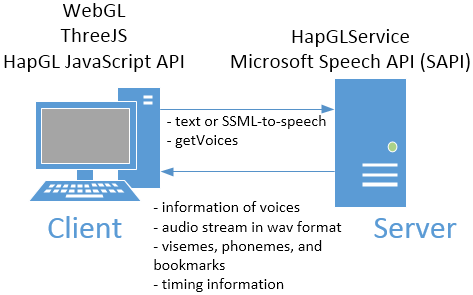
\includegraphics{architecture.png}}
\caption{HapGL architecture.}
\label{architecture}
\end{figure}


\begin{lstlisting}
string GetVoices();

string SpeakText(string text, string voice, 
	         string audioFormat);

string SpeakSSML(string ssml, string voice, 
	         string audioFormat);
\end{lstlisting}

The GetVoices() operation returns a list of the SAPI voices installed in the server, the information
of each voice contains the name, gender, age and culture. Both SpeakText() and SpeakSSML() operations
returns a structure with:
\begin{itemize}
\item The audio stream in wav or mp3 format in a base64 string
\item The sequence of visemes, where each viseme contains the viseme number, the audio position in 
milliseconds, and the duration in milliseconds
\end{itemize}

The difference between SpeakText() and SpeakSSML() is that the first one only accepts a plain input
string and synthesizes using the default options, whereas SpeakSSML() accepts a string in SSML. Voice 
manipulation is specified in SSML by using the \texttt{<prosody>} elements and specifying parameters 
such as: volume, rate and pitch \cite{SSML:Online}. The information returned by these operations are sufficient for the 
lip-synchronization algorithm to generate the sequence of viseme transitions aligned with the audio 
stream. Fig \ref{HapGLService} shows the package diagram for the HapGLService subsystem.

\begin{figure}
\centering
\scalebox{0.55}{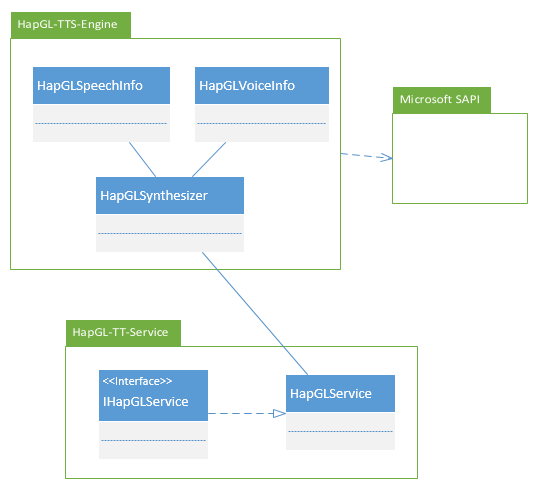
\includegraphics{HapGLService.png}}
\caption{HapGLService package diagram.}
\label{HapGLService}
\end{figure}

HapGL requires to instantiate a \texttt{HapGL()} which expects the URL of the TTS, the mesh of the 
3D character and the mesh of the hair, for example:

\begin{lstlisting}
// Using ThreeJS, load character and 
// hair into mesh1 and mesh2 respectively

var hapgl = HapGL.init({ 
	ttsUrl: 'http://localhost:88/',
	character: mesh1,
	hair: mesh2
});
\end{lstlisting}


\begin{lstlisting}
// Example to activate an Action Unit
hapgl.setAU(`AU1', 100);
\end{lstlisting}

\begin{figure}
\centering
\scalebox{0.8}{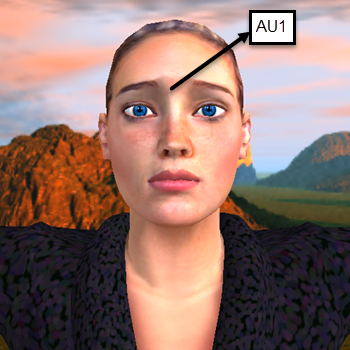
\includegraphics{AU1_100_label.png}}
\caption{Result of setting AU1 to 100 intensity.}
\label{AU1_100}
\end{figure}

\subsubsection{Activating EmFACS emotions with HapGL}
%
Generating emotions in HapGL was done also in the same manner as in HapFACS.
Emotion FACS (EmFACS) introduces a mapping of subsets of action units to
universal emotion identified by Ekman \cite{Ekman:1983} namely fear, anger,
surprise, disgust, sadness, and happines. The emotions implemented in HapGL
were:
\begin{itemize}
\item Happines, combining AU6, AU12, and AU25
\item Sadness, combining AU1, AU4, and AU15
\item Surprise, combining AU1, AU2, AU26, and AU5
\item Anger, combining AU4, AU5, AU7, AU23, and AU24
\item Disgust, combining AU9, AU15, and AU16
\end{itemize}

The current version of HapGL provides three methods related to the speaking 
portion:
\begin{itemize}
\item \texttt{getVoices(function getVoicesCallback)}
\item \texttt{speak(String text, String voice)}
\item \texttt{speakssml(String ssml, String voice)}
\end{itemize}

\texttt{getVoices(function getVoicesCallback)} returns a JSON object with an 
array of voices and will immediately call the \texttt{getVoicesCallback} function with
the result. Since the HapGLService uses Microsoft Speech API (SAPI), the voices are
SAPI-compatible installed on the web-server. More sophisticated voices can be
purchased and installed separately. The following is an example 
of the result of calling \texttt{getVoices}: 

\begin{lstlisting}
hapgl.getVoices(function(output) {...});

// Example of voices returned
{
   voices : [{
      id : "MS-Anna-1033-20-DSK",
      age : "Adult",
      name : "Microsoft Anna",
      gender : "Female",
      culture : "en-US"
   }]
}
\end{lstlisting}

\texttt{speak} and \texttt{speakssml} are similar, the only difference is that
\texttt{speak} will only accept a plain string, whereas \texttt{speakssml} can
accept a string in SSML format as input \cite{SSML:Online}. The \texttt{voice} parameter corresponds
to the \emph{name} attribute of the voices returned by \texttt{getVoices}, if no
\texttt{voice} is passed in then the HapGLService will synthesize using the default
voice in the TTS Server. The \emph{ssml} string argument for the \texttt{speakssml()} function
should be a well-formed SSML Version 1.0 \cite{SSML:Online}. SSML allows
to manipulate the voices by modifying parameters such as: \emph{volume}, \emph{rate},
and \emph{pitch} in the \texttt{<prosody>} elements. Several \texttt{<prosody>} elements
can be combined to produce the desired pronunciation of sentences.

The output of \texttt{speak(..)} and \texttt{speakssml(..)} contains the necessary
information to render the sequence of viseme transitions synchronized with the audio
stream to produce a realistic talking virtual human. The following example shows the
output when speaking the word ``Hello".

\begin{lstlisting}
hapgl.speak(``Hello");

// The output of speaking ``Hello"
{
    audioFormat: ``data:audio\/wav;base64",
    audioStream: ``...",
    visemes: [{
       number : 0,   // silence
       audioPosition : 0.0,
       duration : 3.0,
       emphasis : 0
   }
}
\end{lstlisting}

The sequence of visemes is already sorted in the correct order to be animated. All this
information is sufficient for the lip-synchronization algorithm to render each viseme
at the correct time. The viseme transitions are done smoothly, otherwise, just displaying
the viseme in its maximum intensity would create an undesired illusion. Each 
viseme transition takes a pair of visemes $V_0$ and $V_1$, where $V_0$ is the starting
viseme and $V_1$ is the ending viseme. To do the transformation $V_0 \rightarrow V_1$ we
consider the duration $d_0$ of $V_0$. In $d_0$ time, $V_0$ ``fades out" and $V_1$
``fades in". By ``fade out" we mean interpolating from $V_0$ by setting the value of the
corresponding morph gradually from 1 to 0 in $d_0$ time. Conversely, ``fade in" means
interpolating to $V_1$ by setting the value from 0 to 1. Each viseme maps to a corresponding 
phoneme, we use the mapping provided by the Microsoft Speech API as seen in 
Table \ref{tab:VisemeMapping}. 

\begin{table}[h]
\tbl{Viseme to phonemes mapping in Microsoft Speech API}{%
\begin{tabular}{|l|l|l|l|}\hline
Viseme &{Phoneme(s)} & {Viseme} & {Phoneme(s)}\\
\hline
0 & silence & 11 & ay \\
1 & ae, ax, ah & 12 & h \\
2 & aa & 13 & r  \\
3 & ao & 14 & l \\
4 & ey, eh, uh & 15 & s, z \\
5 & er & 16 & sh, ch, jh, zh \\
6 & y, iy, ih, ix & 17 & th, dh \\
7 & w, uw & 18 & f, v \\
8 & ow & 19 & d, t, n \\
9 & aw & 20 & k, g, ng \\
10 & oy & 21 & p, b, m \\
\hline
\end{tabular}}
\label{tab:VisemeMapping}
\end{table}

Since not all the phonemes have its corresponding Haptek morph register, we choose 
the most similar morph. We used the following viseme to morph mapping in HapGL:

\begin{lstlisting}
var visemeMorphMapping = {
  `0': {name: `neutral'}, `11': {name: `aa'},
  `1': { name: `aa' }, `12': { name: `ih' },
  `2': { name: `aa' }, `13': { name: `n' },
  `3': { name: `aa' }, `14': { name: `n' },
  `4': { name: `ey' }, `15': { name: `s' },
  `5': { name: `er' }, `16': { name: `ch' },
  `6': { name: `ih' }, `17': { name: `th' },
  `7': { name: `uw' }, `18': { name: `f' },
  `8': { name: `ow' }, `19': { name: `d' },
  `9': { name: `aa' }, `20': { name: `g' },
 `10': { name: `ow' }, `21': { name: `m' }	
};
\end{lstlisting}

\begin{table}[h]
\tbl{AUs with recognition rate of less than 100\%. Taken from HapFACS \cite{hapfacs:2013}.}{%
\begin{tabular}{|l|c|l|c|}\hline
AU &{Recognition Rate} & {AU} & {Recognition Rate}\\
\hline
10 & 66.67\% & 16 & 33.33\% \\
11 & 66.67\% & 20 & 66.67\% \\
12 & 66.67\% & 23 & 33.33\%  \\
13 & 66.67\% & 25 & 33.33\% \\
14 & 66.67\% & 28 & 33.33\% \\
\hline
\end{tabular}}
\label{tab:AUrecognitionRate}
\end{table}

\begin{table}[h]
\tbl{AUs comparisson between HapGL and HapFACS.}{%
\begin{tabular}{|l|c|c|}\hline
AU & {HapGL} & {HapFACS}\\
\hline
AU1 & 
\begin{minipage}{.18\textwidth}
  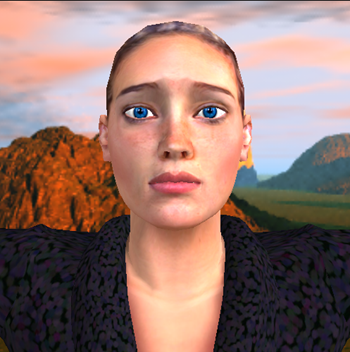
\includegraphics[width=\linewidth]{AU1_100}
\end{minipage}
& 
\begin{minipage}{.18\textwidth}
  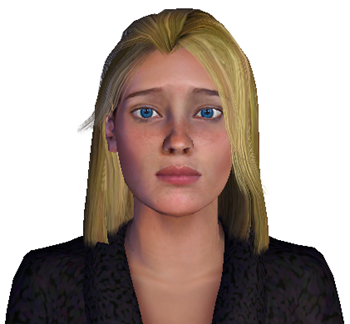
\includegraphics[width=\linewidth]{hp_AU1_100}
\end{minipage} \\
AU5 & 
\begin{minipage}{.18\textwidth}
  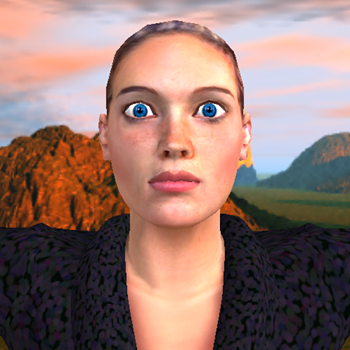
\includegraphics[width=\linewidth]{AU5_100}
\end{minipage}
& 
\begin{minipage}{.18\textwidth}
  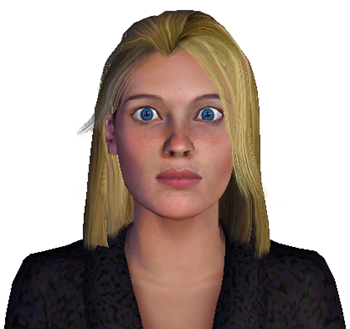
\includegraphics[width=\linewidth]{hp_AU5_100}
\end{minipage} \\
AU17 & 
\begin{minipage}{.18\textwidth}
  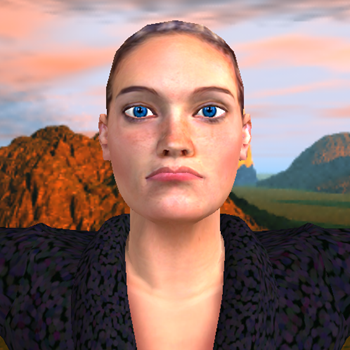
\includegraphics[width=\linewidth]{AU17_100}
\end{minipage}
& 
\begin{minipage}{.18\textwidth}
  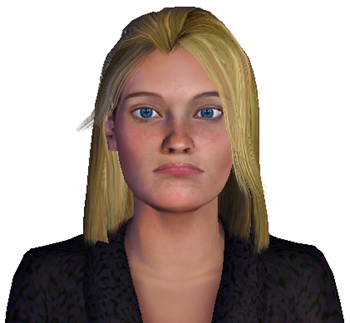
\includegraphics[width=\linewidth]{hp_AU17_100}
\end{minipage} \\
AU18 & 
\begin{minipage}{.18\textwidth}
  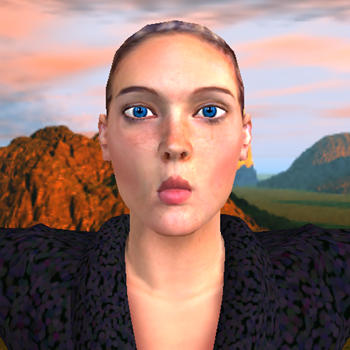
\includegraphics[width=\linewidth]{AU18_100}
\end{minipage}
& 
\begin{minipage}{.18\textwidth}
  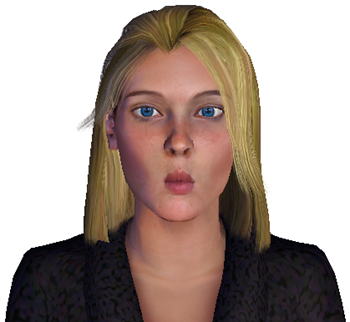
\includegraphics[width=\linewidth]{hp_AU18_100}
\end{minipage} \\
\hline
\end{tabular}}
\label{tab:auevaluation}
\end{table}

\clearpage
To evaluate the lip-synchronization mechanism, we used the Microsoft Speech API
voices installed by default in \textbf{Windows 8.1 x64}: ``David" (Male, en-US), ``Hazel" (Female, en-GB),
and ``Zira" (Female, en-US), however, the results were identical with the three
voices. We first evaluated HapGL with a set of $231$ words, and for each viseme we recorded the
time position in milliseconds where it was displayed and compared to the audio position
returned by the HapGLService and the average difference was $\approx 10ms$, which is acceptable because
"appropriate A/V sync limits have been established and the range that is considered acceptable 
for film is $+/- 22 ms$. The range for video, according to the ATSC, is up to $15 ms$ lead time and 
about $45 ms$ lag time" \cite{Kudrle:2011}. This is a complete list of the randomly-generated words used
int this test:

\begin{quotation}
\emph{Adult, Aeroplane}
\end{quotation}
A similar test was done but with sentences instead. We tested 12 sentences and also obtained the
same result of $\approx 10ms$. Below is the complete list of sentences:
\begin{itemize}
\item \emph{``The quick, brown fox, jumps over the lazy dog."}

\end{itemize}

Then, we chose 4 paragraphs and also achieved the same result of $\approx 10ms$ difference
between the audio position where the viseme was displayed and the actual time. Although this is also a
satisfactory result, for long texts the HapGLService takes several seconds to synthesize the
entire input, and more than $2$ to $3$ \emph{seconds} might be unacceptable on most real-time dialog systems. 
The following example is of one the paragraphs used in this part of the evaluation:

\begin{quotation}
\emph{``I have this fear. It causes my legs to shake.."} \cite{narratives:Online}
\end{quotation}

Similar tests were performed using the default SAPI voice "Microsoft Anna" installed in \textbf{Windows 7 x64}
and \textbf{Windows Server 2008}, and there were noticeable differences between the audio and visemes, for example, in 
words like \emph{well} and \emph{cry}. Therefore, for production systems we would recommend to install
the HapGLService in \textbf{Windows Server 2012} as the default SAPI voices are more natural and the timing
information is more accurate, or to purchase more sophisticated third-party voices compatible with \textbf{Windows 7}
or \textbf{Windows Server 2008}.

\section{Conclusion}
\label{sec:conclusion}
%

Nevertheless, HapGL is still far from being used in production systems as it lacks of other necessary 
functionalities which could be part of future works. To name some, and not intended to be a comprehensive list,
we suggest the following:

\begin{itemize}
\item \emph{Detailed Evaluation}, due to time constraints, a thorough evaluation could not be performed. We suggest
to measure the \emph{believability} of the system by surveying a random sample of users, preferably greater than 20.
Although this is a subjective measure, a user study is still a good indication about the quality of the system.
\end{itemize}

% Bibliography
\bibliographystyle{ACM-Reference-Format-Journals}
\bibliography{malware-bibfile}

\end{document}
% End of v2-acmtog-sample.tex (March 2012) - Gerry Murray, ACM
